\section{Model Abstractrion with Simulation Relations}
\label{sec:abstraction}

As we discussed in \cref{sec:overview}, to further reduce the optimization program~\eqref{eq:averaged-optim}, we employ the notion of model abstraction and simulation relations.
We first distinguish model abstraction and model order reduction.
Model order reduction is a common technique in control theory to reduce the order of a large-scale system so that it becomes manageable. The reduced model, however, still has
the same input and output as the original model. Under the same input signal,
the reduced model should produce an output signal which approximates that of
the original model, within some error bound. The left diagram in
\cref{fig:reduction-vs-abstraction} illustrates this concept, where
$\mathcal{M}_2$ is a reduced-order model of $\mathcal{M}_1$. On the other
hand, model abstraction derives a new model, usually of a lower order, with
completely different input and output than the original model. However, there
exists a relation between the states of the two models that can be maintained
along their evolutions. In other words, one model can track the behavior of
the other under this relation. The right diagram in
\cref{fig:reduction-vs-abstraction} depicts two models with a symbolic
relation $\mathcal{R}$ between their states. If for any admissible input $u_2
(\cdot)$ to $\mathcal{M}_2$ there exists an admissible input $u_1 (\cdot)$ to
$\mathcal{M}_1$ so that the state relation is always maintained along the
traces of the two models, we have a model abstraction. Furthermore, we may
require that a symbolic relation $\mathcal{R}_y$ between their outputs (observations) is also
maintained. A nice property of model abstraction is that we can design a
controller for $\mathcal{M}_1$ by first designing a supposedly simpler
controller for $\mathcal{M}_2$ and then refining it for $\mathcal{M}_1$ using
the symbolic state relation.

\begin{figure}[tb]
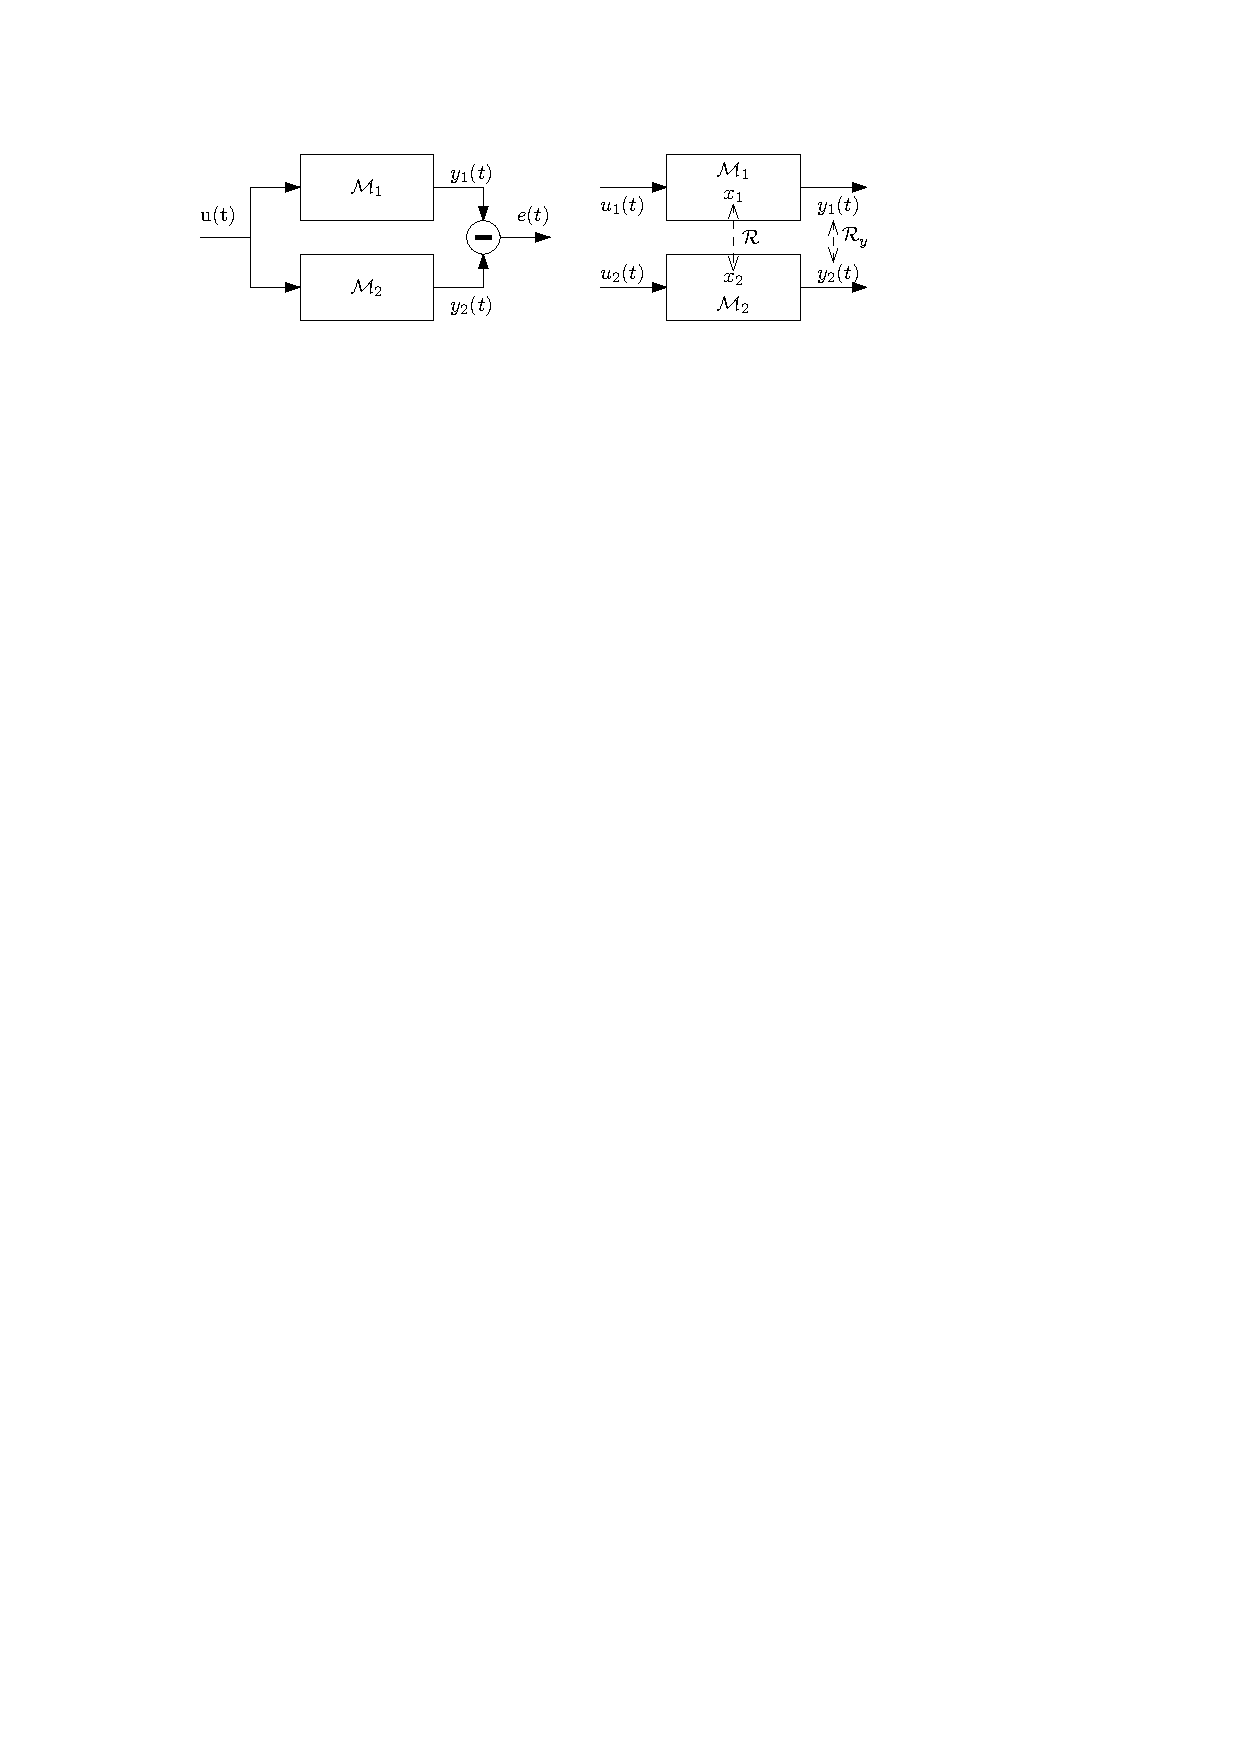
\includegraphics[width=\columnwidth]{abstraction_vs_reduction}
\caption{\label{fig:reduction-vs-abstraction}Model abstraction (right) is
  different from model order reduction (left).}
\end{figure}

\subsection{Simulation Relations between Transition
Systems}\label{sec:abstraction:simulation}

In this section we review the concept of simulation relations between
transition systems. The readers are referred to \cite{girardetal07amd,aluretal00dah} for more thorough treatments of the subject.

The framework of transition systems allows us to unify the modeling of
discrete and continuous, deterministic and non-deterministic dynamical
systems. As we do not concern with the observable outputs of the systems in
this paper, we remove the observation aspect from the definition of transition
systems in {\cite{girardetal07amd}}:

\begin{definition}[Transition System, {\cite{girardetal07amd}}]
  \label{thm:transition-systems-def}
  A transition system is a tuple $T = (Q, \Sigma, \rightarrow, Q^0)$ that
  consists of
  \begin{itemize}
  \item a possibly infinite set $Q$ of states;
  \item a possibly infinite set $\Sigma$ of labels;
  \item a transition relation $\rightarrow \subseteq Q \times \Sigma \times
    Q$;
  \item a possibly infinite set $Q^0 \subseteq Q$ of initial states.
  \end{itemize}
\end{definition}

A transition from state $q$ to state $q^+$ under the label $\sigma$, {\ie}
$(q, \sigma, q^+) \in \rightarrow$, is denoted $q \xrightarrow{\sigma} q^+$.
We assume that the transition systems are {\emph{nonblocking}}, meaning that
for all $q \in Q$, there exists at least one transition starting from $q$. If
for any $q \in Q$ and any $\sigma \in \Sigma$, there is at most one transition
$q \xrightarrow{\sigma} q^+$ of $T$ and $Q^0$ is a singleton, then $T$ is
called {\emph{deterministic}}. Otherwise, it is called
{\emph{nondeterministic}}.

\begin{example}
  The framework of transition systems generalizes dynamical systems. As an
  example, consider a nonlinear discrete-time dynamical system $x^+ = f (x,
  u)$ where $x \in \mathbbm{R}^n$ is the state and $u \in \mathbbm{R}^m$ is
  the input, with initial state $x_{0}$.
  This system can be represented by a deterministic transition
  system $T$ with $Q =\mathbbm{R}^n$, $\Sigma =\mathbbm{R}^m$,
  $\rightarrow = \{ (x, u, x^+) |x \in Q, u \in \Sigma, x^+ = f (x, u) \in Q
  \}$, and $Q^{0} = \{x_{0}\}$.
  If the system is subject to disturbance: $x^+ = f (x, u, w)$ where
  $w \in \mathcal{W} \subseteq \mathbbm{R}^p$ is the disturbance, then $T$
  becomes nondeterministic where $\rightarrow = \{ (x, u, x^+) |x \in Q, u \in
  \Sigma, w \in \mathcal{W}, x^+ = f (x, u, w) \in Q \}$.
\end{example}

A simulation relation between two transition systems $T_1 = (Q_1, \Sigma_1,
\rightarrow_1, Q^0_1)$ and $T_2 = (Q_2, \Sigma_2, \rightarrow_2, Q^0_2)$ is a
stronger notion of system refinement, which allows one system to ``track'' the
other system while maintaining a certain relation between their states. A
simulation relation is defined in \cref{def:simulation-relation}. Note that in
\cite{girardetal07amd}, it is required that $T_1$ and $T_2$ have the same
label sets (and the same observation sets), however we modify the definition
to relax this requirement, \ie $\Sigma_1$ and $\Sigma_2$ can be different.

\begin{definition}[Simulation]
  \label{def:simulation-relation}A relation $\mathcal{R} \subseteq Q_1 \times
  Q_2$ is called a simulation relation of $T_1$ by $T_2$ if and only if for all $(q_1,
  q_2) \in \mathcal{R}$ and for all transitions $q_1 \xrightarrow{\sigma_1}_{1}
  q^+_1$, there exists a transition $q_2 \xrightarrow{\sigma_2}_{2}
  q^+_2$ such that $(q_1^+, q_2^+) \in \mathcal{R}$.
\end{definition}

$T_2$ is said to simulate $T_1$, denoted $T_1 \preceq T_2$, if there exists a
simulation relation $\mathcal{R}$ of $T_1$ by $T_2$ such that for all $q_1 \in
Q^0_1$, there exists $q_2 \in Q^0_2$ such that $(q_1, q_2) \in \mathcal{R}$.
Intuitively, if $T_1 \preceq T_2$ then every state trajectory of $T_1$ can be
``tracked'' by $T_2$ with respect to the state relation $\mathcal{R}$.
Simulation relations and their variants are a powerful tool for safety verification and
hierarchical controller design \cite{clarkeetal99m,pappasetal00hcc,GirardEtAl06vus,girardetal07amd}.

\subsection{Input-Constrained Simulation Relations}
\label{sec:abstraction:ext-simulation}

Conventionally, simulation relations as defined in \cref{sec:abstraction:simulation} do not explicitly take into account %state constraints and
disturbances.  Moreover, there is no relation between the inputs (or labels) to the two systems as required for the total demand bound in our problem.  Therefore, this section extends the concept of simulation relations to account for these ingredients.

\begin{remark}
  For nondeterministic systems, the simulation relation as defined in
  \cref{def:simulation-relation} is not robust to the
  nondeterminism. In particular, it is implicitly assumed that the transition
  from any $q_1$ under any $\sigma_1$, although nondeterministic, is
  detectable so that an appropriate transition $q_2 \xrightarrow{\sigma_2}
  q^+_2$ can be selected. $T_2$ is not nondeterministic anymore because here
  $q_2 \xrightarrow{\sigma_2} q^+_2$ can be chosen to satisfy $(q_1^+, q_2^+)
  \in \mathcal{R}$. Furthermore, it assumes no correlation between the
  nondeterminism of the two systems. In reality, their nondeterminism may be
  correlated, for example if they are subject to the same disturbances in
  different ways. Our extended definition of simulation relations provides
  options for robustness to disturbances and nondeterminism correlation.
\end{remark}

\begin{remark}
  A relation between the labels of $T_1$ and $T_2$ generalizes the simulation
  relation definition in {\cite{girardetal07amd}}, where $\sigma_1$ and
  $\sigma_2$ are related by $\sigma_1 = \sigma_2$ (provided that $\Sigma_1 =
  \Sigma_2$).
\end{remark}

In this section, we generalize the label $\sigma$ of a transition system $T$ as a pair $\sigma = (\upsilon, \delta)$ of a control label $\upsilon \in \mathcal{U}$ and a disturbance label $\delta \in \mathcal{D}$.
Here, $\mathcal{U}$ and $\mathcal{D}$ are respectively the (possibly infinite) sets of control labels and disturbance labels.
The definition of the transition relation is modified accordingly as $\rightarrow \subseteq Q \times \mathcal{U} \times \mathcal{D} \times Q$, and a transition $(q, \upsilon, \delta, q^{+}) \in \rightarrow$ is denoted $q \xrightarrow{(\upsilon, \delta)} q^{+}$.
%The label set $\Sigma$ in \cref{thm:transition-systems-def} is the product $\mathcal{U} \times \mathcal{D}$.
%A transition system is also augmented with a state constraint $Q^S \subseteq Q$ and a mixed constraint $\mathcal{Y} \subseteq Q \times \mathcal{U}$.
Given two transition systems $T_{1}$ and $T_{2}$, we impose a constraint between their control labels $\upsilon_{1}$ and $\upsilon_2$ as a relation $\mathcal{R}_u \subseteq \mathcal{U}_1 \times \mathcal{U}_2$, and a constraint between their disturbance labels $\mathcal{R}_{d}\subseteq \mathcal{D}_1 \times \mathcal{D}_2$.
Note that the constraint $\mathcal{R}_{u}$ is desirable but not required for the execution of the transition systems, \ie an admissible execution of the transition systems may violate the constraint.
The relation $\mathcal{R}_{d}$ takes effect whenever $T_{1}$ and $T_{2}$ are executed simultaneously in the same environment.
%In the following, $\mathcal{P}^{+}(S)$ denotes the set of all non-empty subsets of a set $S$, \ie the superset of $S$ excluding $\emptyset$.
For system $T_{i}$, the set of all admissible successor states from a state $q_{i}$ under label $\sigma_{i} = (\upsilon_{i}, \delta_{i})$ is denoted by $\operatorname{succ}_{i}(q_{i}, \upsilon_{i}, \delta_{i}) = \{q_{i}^{+} \,|\, (q_{i}, \upsilon_{i}, \delta_{i}, q_{i}^{+}) \in \rightarrow_{i}\}$.

\begin{definition}[Input-constrained Simulation]
  \label{thm:ex-simulation-relation}
  % A pair $(\mathcal{R}, \mathcal{R}_{c}$ of a relation $\mathcal{R} \subseteq Q^{S}_1 \times Q^{S}_2$ and a map $\mathcal{R}_{c}: \mathcal{U}_{2} \to \mathcal{P}^{+}(\mathcal{R})$ 
  A relation $\mathcal{R} \subseteq Q^{S}_1 \times Q^{S}_2$ is an input-constrained simulation relation of $T_1$ by $T_2$ if and only if for all $(q_1, q_2) \in \mathcal{R}$ and all $(\upsilon_{1}, \delta_{1}) \in \mathcal{U}_{1} \times \mathcal{D}_{1}$ such that $\operatorname{succ}_{1} (q_{1}, \upsilon_{1}, \delta_{1}) \neq \emptyset$, there exists $\upsilon_{2} \in \mathcal{U}_{2}$ such that
    \begin{enumerate}
    \item $(\upsilon_{1}, \upsilon_{2}) \in \mathcal{R}_{u}$; and
    \item for all $\delta_{2} \in \mathcal{D}_{2}$ such that $(\delta_{1}, \delta_{2}) \in \mathcal{R}_{d}$, $\operatorname{succ}_{2} (q_{2}, \upsilon_{2}, \delta_{2}) \neq \emptyset$ and $(q_{1}^{+}, q_{2}^{+}) \in \mathcal{R}$ %_{c}(\upsilon_{2})$
      $\forall (q_{1}^{+}, q_{2}^{+}) \in \operatorname{succ}_{1} (q_{1}, \upsilon_{1}, \delta_{1}) \times \operatorname{succ}_{2} (q_{2}, \upsilon_{2}, \delta_{2})$.
    \end{enumerate}
\end{definition}


The existence of an input-constrained simulation relation $\mathcal{R}$ of $T_{1}$ by $T_{2}$ allows $T_{2}$ to track any state sequence of $T_{1}$ with respect to $\mathcal{R}$, as long as their initial states are in $\mathcal{R}$.
We define a trajectory of $T_{i}$ as a (potentially infinite) sequence of admissible states, labels, and transitions: $q_{i}^{0} \xrightarrow{\upsilon_{i}^{0}, \delta_{i}^{0}}_{i} q_{i}^{1} \xrightarrow{\upsilon_{i}^{1}, \delta_{i}^{1}}_{i} q_{i}^{2} \cdots$.
The next lemma follows directly from the \cref{thm:ex-simulation-relation}.
It essentially says that if an input-constrained simulation relation $\mathcal{R}$ of $T_{1}$ by $T_2$ exists then $T_{2}$ can be controlled to track any admissible trajectory of $T_{1}$, with respect to $\mathcal{R}$, while keeping the input constraint $\mathcal{R}_{u}$.

\begin{lemma}
  \label{thm:ex-simulation-tracking}
  Suppose $\mathcal{R}$ is an input-constrained simulation relation of $T_{1}$ by $T_{2}$, whose initial states satisfy $(q_{1}^{0}, q_{2}^{0}) \in \mathcal{R}$.
  Let $\kappa_{2}: Q_{1} \times \mathcal{U}_{1} \times \mathcal{D}_{1} \times Q_{2} \to \mathcal{U}_{2}$ be any feedback law such that for all admissible quadruples $(q_{1}, \upsilon_{1}, \delta_{1}, q_{2}) \in Q_{1} \times \mathcal{U}_{1} \times \mathcal{D}_{1} \times Q_{2}$, $\upsilon_{2} = \kappa_{2} (q_{1}, \upsilon_{1}, \delta_{1}, q_{2})$ satisfies the conditions in \cref{thm:ex-simulation-relation}.
  Such a feedback law always exists.
  Then for any trajectory of $T_{1}$, %(respectively, $\upsilon_{2}^{k} = \rho_{2} (q_{1}^{k}, \upsilon_{1}^{k}, q_{2}^{k})$)
  any corresponding trajectory of $T_{2}$ with $\upsilon_{2}^{k} = \kappa_{2} (q_{1}^{k}, \upsilon_{1}^{k}, \delta_{1}^{k}, q_{2}^{k})$ satisfies $(q_{1}^{k}, q_{2}^{k}) \in \mathcal{R}$ and $(\upsilon_{1}^{k}, \upsilon_{2}^{k}) \in \mathcal{R}_{u}$ for all $k$.
\end{lemma}

%%% Local Variables:
%%% mode: latex
%%% TeX-master: "emsoft15gs"
%%% End:
